\section{Livello 4: Transport}
    \subsection{Scopo e panoramica del livello}
        Il livello \textit{trasporto}, si occupa di fornire al livello applicazione paradigmi astratti per la comunicazione tra due processi: flusso di byte, scambio di messaggi, chiamate a funzione, etc.

        Offre al livello applicativo un'interfaccia indipendente dalle diverse tecnologie dello strato di rete (IPv4, IPv6).

        Per assolvere le sue funzioni, utilizza i servizi offerti dallo strato di rete.

        Ci sono dei presupposti della rete sottostante da tenere in considerazione: i messaggi potrebbe andare perduti, potrebbero arrivare con un ordine modificato, potrebbe essercene più copie, potrebbe esserci ritardi indefiniti.

        I servizi di trasporto si basano sulla \textbf{Socket Library} introdotta dall'Università di Berkeley nel 1982. Fornisce due tipi di servizio di trasporto:
        \begin{itemize}
            \item Servizio affidabile orientato alla connessione: \textbf{stream sockets (TCP)}, offre garanzia di intergrità, completezza ed ordine. Gli utenti TCP vedono la connessione come una pipe.
            \item Servizio inaffidabile di datagrammi: \textbf{datagram sockets (UDP)}; ogni blocco di dati viene inviato e ci si dimentica di esso.
        \end{itemize}

        Nel processo di ricezione dei pacchetti di livello rete (\textbf{demultiplexing}) il livello di trasporto deve analizzare la porta di destinazione e smistare di conseguenza il pacchetto a livello applicativo.

        Nel processo di spedizione dei dati (\textbf{multiplexing}), il dato viene eventualmente ridotto in segmenti, detti anche \textbf{Transport Data Protocol Unit (TPDU)}, che vengono imbustati nell'header di trasporto con l'indicazione della porta di destinazione.

        \begin{center}
            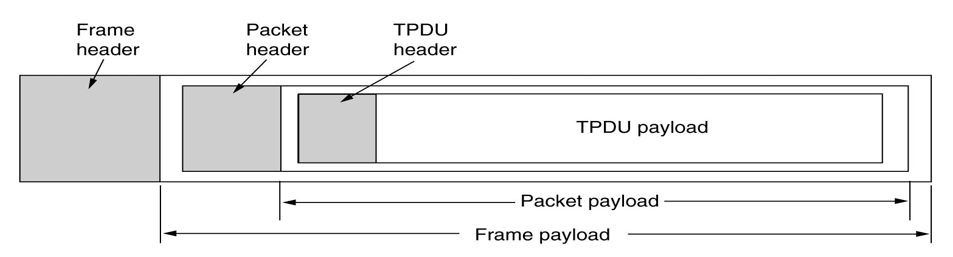
\includegraphics[scale=0.36]{chapters/5/assets/schema_a.png}
        \end{center}

        La porta è un identificativo numerico (16 bit, 64K porte) che rappresenta il punto di arrivo di una connessione con un host.

        La coppia (IPaddr, Port) identifica univocamente un estremo della connessione, ed è detta \textbf{socket}.

        Ogni connessione è quindi identificata da una coppia di socket.

        Le porte inferiore a 1024 sono dette \textbf{Well Know Port}, e vengono universalmente associate a determinate applicazioni server da \textbf{IANA}, per agevolare l'identificazione del socket server.

        \subsubsection{Identificazione delle porte}
            Se il servizio è standard, il server utilizza una Well Know Port che tutti conoscono, altrimenti per servizi di rete dinamici, si utilizza un \textbf{Name Server} con un servizio di \textbf{PortMapper} in ascolto su una Well Know Port, su cui i servizi di rete registrano la porta in ascolto (1). Il client interroga il \textit{PortMapper} per conoscere la porta del server (2), quindi contatta il server (3).
        
            Questo meccanismo è utilizzato dal protoccolo RPC.

            \begin{center}
                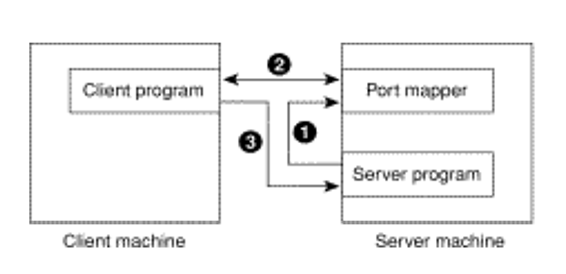
\includegraphics[scale=0.45]{chapters/5/assets/schema_b.png}
            \end{center}

        \subsubsection{Segmentazione dei dati}
            Il mittente può scegliere la dimensione massima del segmento, \textbf{Max Segment Size (MSS)} in base a parametri quali il buffer di trasmissione o l'\textit{MTU} dell'interfaccia locale meno i byte dell'header TCP/UDP ed i byte dell'header IP.
        
            I segmenti vanno consegnati al layer Network (IP) il quale si occuperà della consegna all'host di destinazione.
        
            Se durante il tragitto si incontra una rete con un MTU inferiore alla dimensione del pacchetto, allora il protocllo IP frammenterà il pacchetto in due o più parti, per poi ricomporle a destinazione.

            \begin{center}
                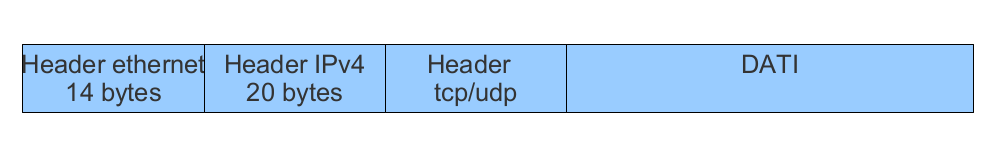
\includegraphics[scale=0.34]{chapters/5/assets/schema_c.png}
            \end{center}

        \subsubsection{Il modello client/server}
            La Berkeley Socket Library utilizza un modello di tipo client/server.
        
            Un estremo server è sempre in ascolto su una porta stabilita, la primitiva \verb:bind(): lega il processo alla porta.
        
            L'altro estremo, client, prenderà contatto il server specificandone la porta, che dovrà essere nota al client. La porta utilizzata dal client apparirà al server nell'intestazione di trasporto, quindi la porta del client non deve essere nota a priori. Generalmente viene determinata dinamicamente dal sistema operativo al momento della richiesta di connessione.
        
            Quando il client invia un messaggio con \verb:sendto():, riceve dal sistema operativo un numero di porta dinamico.
        
            All'eventuale successivo \verb:recvfrom():, il client si mette in ascolto sulla stessa porta, nota al server perché contenuta nel messaggio.
        
            Il server inizia con un \verb:recvfrom(): e la sua porta in ascolto deve essere stabilita dall'applicazione mediante la primitiva \verb:bind():.

            \begin{center}
                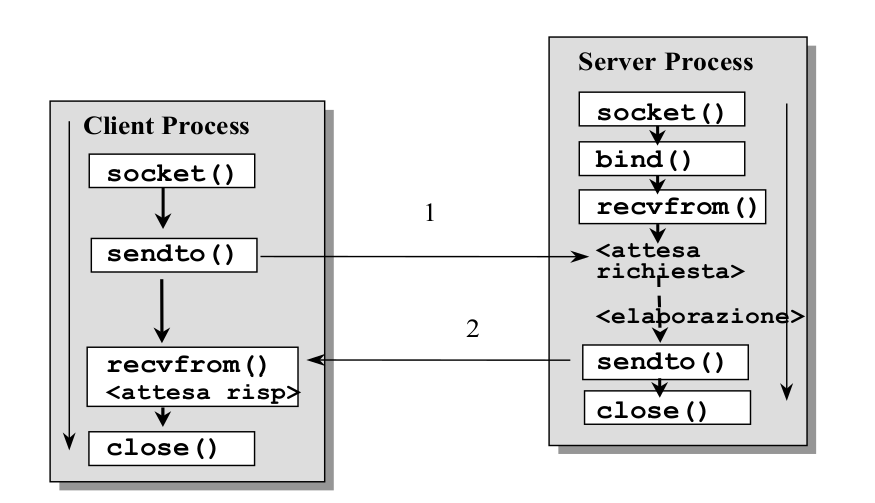
\includegraphics[scale=0.38]{chapters/5/assets/schema_d.png}
            \end{center}

        \subsubsection{Protocollo TCP}
            Per servizi connection-oriented (TCP), la libreria fornisce la primitiva \verb:listen(): che predispone le code di attesa per i processi client che accederanno contemporaneamente al servizio; e la primitiva bloccante \verb:accept(): che consente al server di mettersi in ascolto sulla porta.
        
            Quando arriva un TPDU il server crea un nuovo socket con le stesse proprietà di quello originale e ritorna un file descriptor per esso.
        
            Il server può creare un nuovo processo tramite \verb:fork(): oppure un nuovo thread per gestire la connessione sul nuovo socket, e tornare ad aspettare la prossima connessione.
        
            La primitiva \verb:connect(): è utilizzata dal client per aprire una connessione. QUando la connessione è instaurata, la distinzione tra client e server non esiste più, ma generalmente, il primo invio dei dati viene fatto dal client con la primitiva \verb:send(): la cui corrispondente \verb:recv(): deve essere attivata dall'altro estremo. In Unix, si possono utilizzare anche le primitive \verb:read(): e \verb:write():.

            \begin{center}
                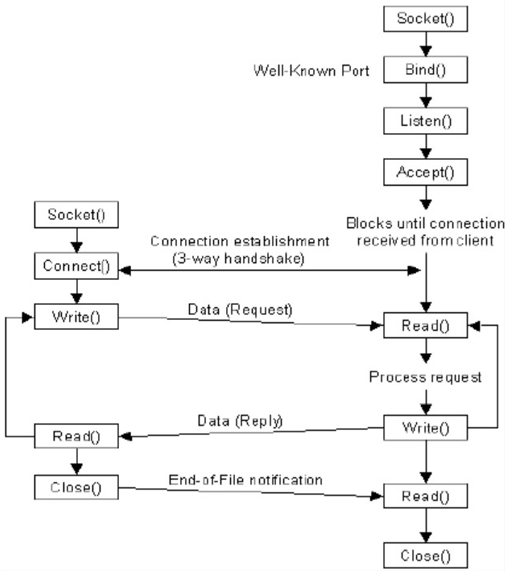
\includegraphics[scale=0.4]{chapters/5/assets/schema_e.png}
            \end{center}

            Il protocollo TCP fornisce un flusso di byte end-to-end affidabile, a partire da un servizio di rete inaffidabile (IP).

            Le connessioni TCP sono del tipo full-duplex e unicast.

            TCP riceve flussi di byte dai processi locali, li spezza in segmenti e li spedisce in datagrammi IP separati.

            L'applicazione che spedisce (write) consegna i dati in un buffer di spedizione.

            I byte possono essere raggruppati (o frazionati) in segmenti da consegnare al livello rete.

            La dimensione massiama dei segmenti è 64K, ma quasi sempre sono di 1460 byte di dati che, con le aggiunte dell'header TCP e IP arriva 1500, che è l'MTU di Ethernet.

            Il flag "PUSH" può essere utilizzato per l'invio non ritardato.

            Il livello TCP di destinazione scrive i segmenti nel buffer di destinazione e consegna all'applicazione (read) tutti i byte riscontrati (ricevuti in ordine), ricostruendo il flusso originale.

        \subsubsection{Protocollo UDP}
            Il protocollo UDP offre alle applicazioni un modo per inviare datagrammi senza stabilire una connessione.
        
            La differenza con TCP è l'aggiunta delle porte di origine e destinazione necessarie per il multiplexing: l'intestazione UDP contiene inoltre la lunghezza del segmento (header più dati) ed il checksum facoltativo che è la somma in complemento a 1 delle sequenze di 16 bit.

            \begin{center}
                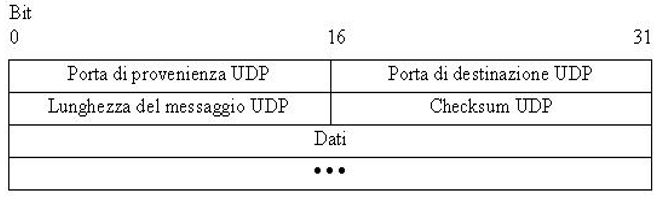
\includegraphics[scale=0.45]{chapters/5/assets/schema_f.png}
            \end{center}

            Il protocllo UDP viene utilizzato per l'implementazione dei protocolli applicativi che richiedono lo scambio di brevi messaggi (DHCP, DNS, TFTP), la costruzione (a livello applicativo) di servizi di trasporto più astratti denominati protocolli middleware (RCP e RTP) e per la comunicazione multicast.

    \subsection{Servizio orientato alla connessione}
        \subsubsection{Corretta consegna ed ordinamento dei segmenti}
            Il riscontro o \textbf{ACKnowledgement} abbinato al numero di sequenza attribuito ad ogni pacchetto dati o ad ogni byte del flusso, rappresentano uno strumento molto utilizzato per la verifica della corretta consegna dei pacchetti e del relativo ordinamento.
        
            TCP utilizza la numerazione dei byte. Il numero iniziale della sequenza non è 0, ma è determinato in modo da evitare che in seguito alla reinizializzazione di una connessione si faccia confusione tra vecchi e nuovi pacchetti.
        
            Il protocollo consiste nei seguenti passi:
            \begin{enumerate}
                \item Il mittente invia un segmento di dati assieme ad un numero progressivo (in TCP è un numero relativo al primo byte del segmento).
                \item Il destinatario invia un pacchetto con un Flag (ACK) attivo ed il numero del segmento ricevuto correttamente (in TCP è il numero del prossimo byte che si aspetta di ricevere).
                \item Il mittente attiva un \textbf{Retransmittion Time Out (RTO)} per ogni segmento inviato, se non riceve un ACK di segmento, ricomincia a spedire dall'ultimo byte riscontrato (GoBack-N).
            \end{enumerate}

            \begin{center}
                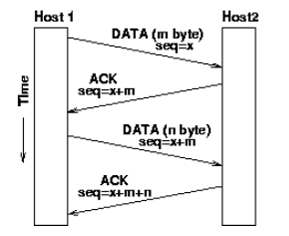
\includegraphics[scale=0.55]{chapters/5/assets/schema_g.png}
            \end{center}

        \subsubsection{Attivazione della connessione}
            Il dialogo tra client e server per l'attivazione di una connessione deve tenere conto dell'inaffidabilità della rete sottostante. Il problema maggiore è dato dai possibili duplicati ritardati che non devono essere confusi con nuove connessioni.
        
            La soluzione proposta da \textbf{Tomlinson} è un meccanismo di \textbf{handshaking a tre vie}:
            \begin{enumerate}
                \item Il client invia un segmento di \textbf{Connection Request (CR)} con un valore iniziale di sequenza.
                \item Il server risponde con un ACK che riscontra il valore di sequenza proposto dal client e propone un valore iniziale di sequenza verso il client.
                \item Il client invia un terzo segmento con ACK, il risconto della sequenza del server ed eventualmente può anche trasportare i primi dati.
            \end{enumerate}

        \subsubsection{Apertura di una connessione in TCP}
            La soluzione in uso in TCP deriva dall'algoritmo di Tomlinson:
            \begin{enumerate}
                \item La \textbf{CONNECT} sul client invia un segmento con \textbf{SYC = 1, ACK = 0, seq = x} (random).
                \item Se il server è in ascolto (\textbf{LISTEN}) ed accetta la connessione, risponde con
                un segmento in cui \textbf{ACK = 1, SYQ = 1, ACKseq = x + 1, seq = y} (random).
                \item Il client termina l'apertura riscontrando la sequenza del server \textbf{ACK = 1, ACKseq = y + 1}.
            \end{enumerate}

            \begin{center}
                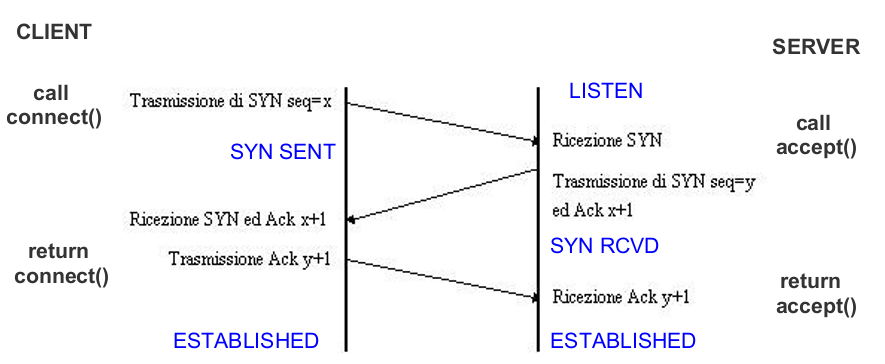
\includegraphics[scale=0.37]{chapters/5/assets/schema_h.png}
            \end{center}

        \subsubsection{Chiusura della connessione TCP}
            Si utilizza un handshaking a due vie per ogni direzione.
        
            Generalmente viene fatto con tre segmenti, inviando il secondo \textbf{FIN} assieme all'ACK. Se una risposta FIN non arriva entro 2RTT, il mittente FIN rilascia la connessione.
        
            La primitiva \verb:close(): determina l'invio del FIN, e marca come chiuso un canale. Il canale non è più utilizzabile con \verb:read(): o \verb:write():.
        
            La primitiva \verb:shutdown(): può chiudure il canale in una direzione.
        
            \textbf{TIME WAIT} attende per 2 \textbf{MSL (Maximum Segment Lifetime)} l'arrivo di eventuali pacchetti ancora in rete, MSL è una stima del tempo di vita di un segmento, in Linux è tipicamente 30 secondi.

            \begin{center}
                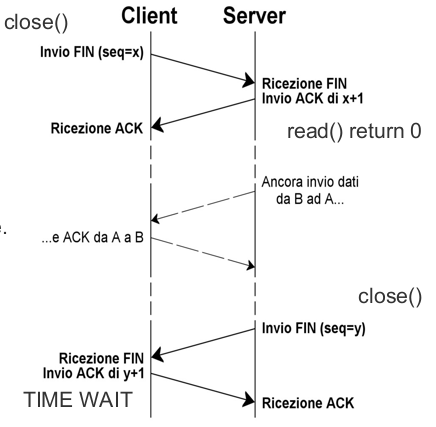
\includegraphics[scale=0.5]{chapters/5/assets/schema_i.png}
            \end{center}

        \subsubsection{Buffering}
            Per ogni connessione TCP è necessario un buffer di trasmissione e di ricezione, implementato come una coda circolare, poiché i segmenti potrebbe essere perduto e/o andate fuori ordine e perché i processi di lettura/scrittura potrebbero lavorare a velocità diverse.
        
            Il buffer di trasmissione contiene i dati spediti ma non ancora riscontrati (tra LastByteSent e LastByteAcked), i dati ancora da spedire (dopo LastByteSent) e dello spazio libero.
        
            Il buffer di ricezione contiene i dati ricevuti e riscontrati ma non ancora letti dall'applicazione, i dati ricevuti ma non ancora riscontrati (cioè i dati ricevuti fuori ordine) e dello spazio libero.
        
            In ambiente Unix, possiamo controllare i buffer attualmente in uso con il comando: \verb:sysctl -a | grep tcp:

            La dimensione del buffer può essere modificata con \verb:setsockopt():: \textbf{SO\_RC\-VBUF} imposta la dimensione del buffer di ricezione, mentre \textbf{SO\_SNDBUF} imposta la dimensione del buffer di trasmissione.

        \subsubsection{Socket non bloccanti}
            La funzione \verb:send(): è per default bloccante, si blocca quando il buffer in trasmissione è pieno e ritorna quando si libera spazio. Se lo spazio è insufficiente, viene effettuata una scrittura in una porzione di dati minore o uguale alla dimensione del buffer libero, e la \verb:send(): restituisce il numero dei byte scritti.
        
            Se il buffer è pieno ed il socket è impostato come non bloccante, non ci sarà nessun blocco, ma ritornerà -1, settando la variabile di errore \textbf{EWOULDBLOCK}.
        
            La funzione \verb:recv(): è per default bloccante, si blocca quando il buffer di ricezione è vuoto, e ritorna quando ci sono dati nel buffer. Il numero di byte letti può essere inferiore al numero di byte richiesto.
        
            Ritorna 0 quando non ci sono dati nel buffere l'altro peer ha chiuso la trasmissione. Se il buffer è vuoto, ed il socket è stato impostato come non bloccante, non ci sarà nessun blocco, ma ritornerà -1 impostando la variabile di errore \textbf{EWOULDBLOCK}.

        \subsubsection{Controllo di flusso: Sliding Window}
            Per il controllo del flusso e l'ottimizzazione del throughput della rete in TCP si utilizza il meccanismo denominato \textbf{Sliding Window (finestra scorrevole)}:
            \begin{itemize}
                \item Il ricevente annuncia la \textbf{Receiver Window Size (rwnd)} al trasmettitore, che generalmente corrisponde al numero di byte liberi sul buffer di ricezione e indica quanti byte possono essere inviati a partire dall'ultimo riscontrato.
                \item Il trasmettitore può inviare anche più dati senza riscontro, purché il numero di byte non riscontrati non ecceda rwnd:
                \begin{equation*}
                    SlidingWindow = LastByteSent - LastByteAcked < rwnd
                \end{equation*}
            \end{itemize}

            Il ricevitore può bloccare la trasmissione (ad eccezione degli \textbf{Urgent Data}) inviando rwnd = 0 (stop-and-wait).

            \begin{center}
                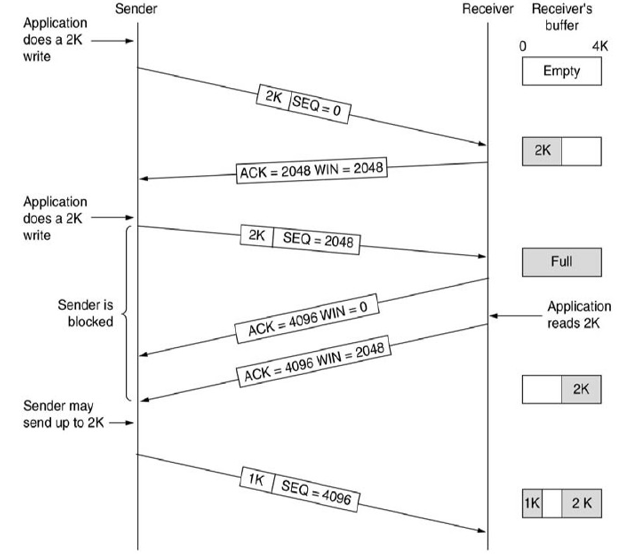
\includegraphics[scale=0.4]{chapters/5/assets/schema_j.png}
            \end{center}

    \subsection{La trama TCP}
        Porta di provenienza e destinazione identificano gli estremi della connessione. Il \textbf{Numero Sequenziale} è il contatore del flusso di byte spediti: indica il numero del primo byte di dati contenuto nel segmento.
    
        Il \textbf{Numero di Riscontro} è il contatore del numero di byte ricevuti: indica il numero del prossimo byte che il destinatario si aspetta di ricevere.
    
        \textbf{HLEN} (parole di 32 bit dell'header) è necessario perché il campo opzioni è variabile.

        \begin{center}
            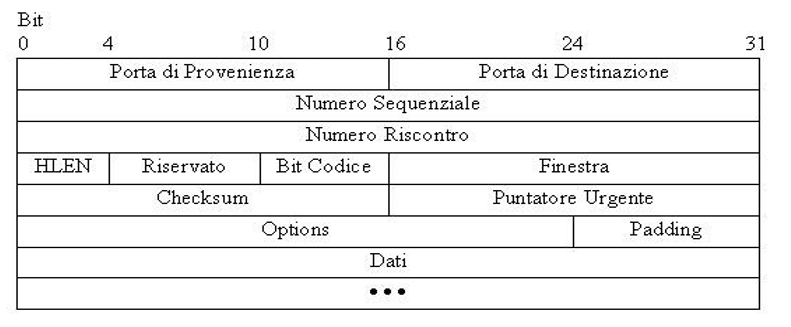
\includegraphics[scale=0.43]{chapters/5/assets/schema_k.png}
        \end{center}

        \subsubsection{La trama TCP: i bit di codice}
            Dopo HLEN ci sono 4 bit riservati per sviluppi futuri, poi abbiamo 8 bit di codice.
        
            Se attivi, cioè settati ad 1, hanno il seguente significato:
            \begin{itemize}
                \item \textbf{CWR e ECE}: vengono utilizzati quando è attivo ECN (gestione della concorrenza).
                \item \textbf{ECE (ECN-Echo)}: usato per mandare ad un host l'indicazione di rallentare.
                \item \textbf{CWR}: è generato dall'host per indicare che ha ridotto la finestra di congestione.
                \item \textbf{URG}: si deve considerare il campo puntatore urgente.
                \item \textbf{ACK}: si deve considerare il numero di riscontro.
                \item \textbf{PSH}: il ricevente non deve bufferizzare, ma renderli subito disponibili all'applicazione.
                \item \textbf{RST}: reset della connessione a causa di un qualche errore.
                \item \textbf{SYN}: utilizzato nella fase di attivazione di una connessione.
                \item \textbf{FIN}: utilizzato nella fase di chiusura di una connessione.
            \end{itemize}

        \subsubsection{La trama TCP: finestra, checksum e puntatore urgente}
            \textbf{Finestra} (16 bit): è la dimensione della Sliding Window, ovvero il numero di byte che il destinatario è in grado di ricevere a partire dall'ultimo byte riscontrato.
        
            La dimensione massima sarebbe di 64KB, ma può essere aumentata attraverso la \textit{scala della finestra}.

            Il \textbf{checksum} (16 bit): somma in complemento a 1 delle sequenze di 16 bit del segmento TCP (header e dati) e della pseudo-intestazione.

            La \textbf{pseudo-intestazione} include ulteriori informazioni importanti di IP e TCP (IP source, IP dest, 0x00, 0x06, TCP Segment length), violando però l'indipendenza dei protocolli perché include dati del Layer IP.

            \textbf{Puntatore urgente} (16 bit): puntatore a dato urgente, ha significato solo se il flag URG è impostato a 1 ed indica lo scostamento in byte dell'ultimo dato urgente. Tipicamente sono messaggi di controllo, usato raramente.

            \begin{center}
                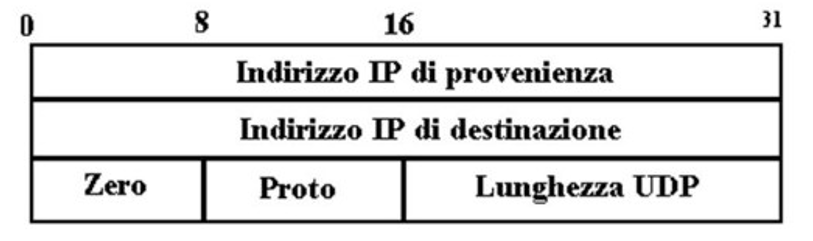
\includegraphics[scale=0.4]{chapters/5/assets/schema_l.png}
            \end{center}

        \subsubsection{La trama TCP: opzioni}
            Ciascun segmento SYN contiene in genere delle opzioni per il protocollo TCP che servono per comunicare all'altro capo una serie di parametri utili a regolare la connessione.
        
            Normalmente vengono usate le seguenti opzioni:
            \begin{itemize}
                \item \textbf{MSS}: massima dimensione del segmento che il destinatario può accettare (è possibile determinare questo valore con l'opzione del socket \textbf{TCP\_MA\-XSEG}).
                \item \textbf{Scala della finestra}: la finestra è normalmente di 16 bit (max 64K). In alcuni casi (alta velocità o alta latenza) questa finestra è insufficiente; in questo caso la Scala determina numero di shift a sinistra (2x) della finestra.
                \item \textbf{SACK}: Selective ACKnowledgement.
                \item \textbf{timestamp}: è un marcatore temporale spedito dal mettente (timestamp value) e imbalzato poi dal destinatario (timestamp echo reply), per il calcolo del RTT. Se concordato, in avvio della connessione viene incluso in ogni segmento.
            \end{itemize}
            
            Se i byte delle opzioni non sono multipli di 4 (parole di 32 bit), viene aggiunto un \textbf{padding} opportuno.

        \subsubsection{Determinazione del MSS ottimale}
            La frammentazione introduce un overhead sull'attività dei router: frammenti troppo piccoli determinano un overhead sul traffico di rete.
        
            L'MSS ottimale è l'MTU minimo tra gli tutti MTU incontrati nel tragitto, ma questo dato non è noto quando si inizia una trasmissione e potrebbe cambiare nel tempo.
        
            L'algoritmo generalmente utilizzato è il seguente:
            \begin{itemize}
                \item Il mittente determina la \textbf{MSS (Maximum Segment Size)} generalmente con la MTU dell'interfaccia locale (meno 20 byte dell'header TCP e 20 dell'header TCP) e lo comunica all'altro host attraverso le opzioni dell'header TCP.
                \item Quindi invia il primo segmento con il bit DF (Don't Fragment) settato a 1. Se durante il cammino si incontra un router con MTU inferiore questo invierà al mittente un pacchetto ICMP di errore che verrà utilizzato per correggere l'MSS.
            \end{itemize}

        \subsubsection{La trama TCP: opzione SACK}
            Normalmente TCP funziona con \textbf{GoBackN}: se il ricevente ottiene un segmento errato e N segmenti validi, il riscontro si ferma all'ultimo valido prima dell'errore.
        
            Questo manda in timeout il mittente che rimanda tutti i segmenti a partire da quello errato.
        
            Per migliorare le prestazioni evitando la ritrasmissione di segmenti validi, è stata proposta la tecnica \textbf{SACK (Selective ACK)}: il ricevitore indica al trasmettitore quali segmenti sono arrivati correttamente, in modo che possa determinare quali segmenti devono essere rispediti.
        
            Funziona con due opzioni dell'header TCP:
            \begin{itemize}
                \item \textbf{SACK Permitted}: viene incluso in un segmento SYN per indicare la capacità di gestire la tecnica SACK.
                \item \textbf{SACK}: utilizzato dal ricevente per comunicare le informazioni SACK (i segmenti ricevuti correttamente).
            \end{itemize}

        \subsubsection{Ottimizzazioni per casi particolari}
            Le prestazioni possono degradare in alcuni casi particolari quali:
            \begin{itemize}
                \item il trasmettitore genera dati lentamente, ad esempio quando si edita un file per ogni tasto premuto girano 4 pacchetti IP per un totale di 162 byte.
                \item il ricevitore consuma dati lentamente; ad esempio il destinatario pubblica finestre di pochi byte, perché l’applicazione legge pochi byte per volta, quindi il mittente è costretto a spezzare il flusso in tanti segmenti (problema della finestra futile).
            \end{itemize}

            Per attenuare il problema lato mittente usa l'\textbf{algoritmo di Nagle}:
            \begin{itemize}
                \item se il mittente ha pochi byte da spedire (a causa dell'applicazione o della finestra del destinatario) e ci sono dati non riscontrati, allora esso aspetta un ACK, ovvero un RTT.
                \item se il mittente ha molti byte da spedire oppure i segmenti piccoli sono riscontrati, allora il mittente spediscie subito.
            \end{itemize}

            Questo algoritmo può essere disabilitato con l'opzione TCP\_NODELAY. Esempio in C: \verb:setsockopt(sock, SOL_TCP, TCP_NODELAY, ...):

            Per attenuare il problema lato ricevente si usa la \textbf{soluzione di Clark}:
            \begin{itemize}
                \item Se il ricevente pubblica finestre troppo piccole, l'algoritmo forza il ricevitore ad attendere che la finestra raggiunga un valore minimo prima di comunicarlo al mittente.
            \end{itemize}

        \subsubsection{Il Retransmission timeout (RTO) di TCP}
            Serve per decidere quando un pacchetto deve considerarsi perduto.
        
            Deve essere almeno pari a RTT, ma deve aggiornarsi dinamicamente e deve gestire situazioni di congestione (backoff).
        
            \textbf{Algoritmo di Jacobson}: se l'ACK torna indietro prima dello scadere dell'RTO, l'algoritmo calcola il valore del RTT (Round Trip Time) e aggiorna due variabili:
            \begin{equation*}
                RTT_{medio} = \alpha \cdot RTT_{medio} + (1 - \alpha) \cdot RTT
            \end{equation*}

            \begin{equation*}
                Dev_{media} = \alpha \cdot Dev_{media} + (1 - \alpha) \cdot |RTT - RTT_{medio}|
            \end{equation*}

            \begin{equation*}
                RTO = RTT_{medio} + 4 \cdot Dev_{media}
            \end{equation*}

            Dove $\alpha$ è il peso che si vuole dare ai precedenti valori medi, tipicamente $\alpha$ = 0.9.

            Per le reti congestionate, si applica l'\textbf{algoritmo di Backoff di Karn}: se l'RTO scade, significa che la rete è congestionata, in questo caso l'algoritmo di Karn prevede di non aggiornare il RTT$_{medio}$, ma raddoppiare l'RTO fino a quando i segmenti non arrivano a destinazione al primo tentativo.

            \begin{equation*}
                RTO(i + 1) = 2RTO(i)
            \end{equation*}

            Rappresenta il backoff medio esponenziale.

        \subsubsection{I timer di TCP in Linux}
            Oltre a RTO, che è il più importante, TCP gestisce altri timer:
            \begin{itemize}
                \item \textbf{Timer di persistenza}: viene attivato quando la finestra viene chiusa (rwnd = 0). Se il pacchetto che riapre va perduto, allo scadere del timer il mittente invia una window probe che sollecita la rispedizione della finestra. Se la finestra è ancora a 0 il timer viene reimpostato.
                \item \textbf{Time wait}: rappresenta tempo di attesa in FIN-WAIT dopo un FIN. Prima di rilasciare la connessione viene attivato questo timer per gestire eventuali pacchetti circolanti dopo la chiusura.
                \item \textbf{Timer di keepalive}: parte quando la linea è inattiva. Se arriva a 0 TCP invia un ACK, se non riceve risposta la connessione viene considerata interrotta.
            \end{itemize}

    \subsection{Controllo della congestione}
        Quando troppi pacchetti sono presenti in una porzione della rete le prestazioni si degradano e la rete si dice \textbf{congestionata}. La congestione ha effetto su tutti i parametri della rete: velocità, ritardo, jitter ed affidabilità.
    
        Per \textbf{controllo della congestione} si intendono le procedure per prevenire la congestione prima che si verifichi (\textbf{controllo proattivo}) o eliminarla quando si è verificata (\textbf{controllo reattivo}).
    
        Coinvolge il comportamento dei terminali (host) e dei nodi di transito (router). Può essere svolto a vari livelli (generalmente a livello rete e a livello trasporto in TCP).

        \subsubsection{Controllo della congestione in TCP}
            In TCP l'host gestisce la congestione mediante l'introduzione di una ulteriore finestra denominata \textbf{Congestion Window (cwnd)}.
        
            La finestra effettivamente utilizzata in trasmissione (\textbf{awnd}) è la finestra più piccola tra la finestra indicata dal ricevente (\textbf{rwnd}) e la finestra di congestione (\textbf{cwnd)}:
            \begin{equation*}
                awnd = min(cwnd, rwnd) \geq LastByteSent - LastByteAcked
            \end{equation*}

            La Congestion Window cwnd dovrà essere regolata mediante opportuni algoritmi (generalmente Slow Start per il controllo proattivo e TCP Reno per il controllo reattivo).

        \subsubsection{Gestione della cwnd: Algoritmo Slow Start}
            Per il controllo proattivo, si utilizza l'algoritmo \textbf{Slow Start}.
        
            Il mittente imposta cwnd = MSS e la raddoppia ad ogni invio fino a quando il cwnd raggiugne la dimensione della finestra del ricevente rwnd, oppure, qunado il cwnd raggiunge una soglia (valore tipico 64 KB). Raggiungendo la \textbf{soglia}, l'aumenta diventa lineare.

            Per il controllo reattivo, si utilizza l'algoritmo \textbf{Tahoe}.
    
            Se scade il timer si ha congestione, quindi si ritorna a Slow Start (cwsd = MSS), la soglia viene impostata a metà del valore corrente di cwnd.
    
            Il crollo repentino del cwnd decongestiona la rete, ma limita temporaneamente la velocità di ricezione e trasmissione dei dati.

        \subsubsection{Controllo reattivo con fast recovery (TCP Reno)}
            TCP Reno migliora il Tahoe distinguendo tra due motivi per la perdita di dati:
            \begin{itemize}
                \item Dovuto al timeout del timer: quindi la rete è molto congestionata, viene impostato cwnd = MSS.
                \item Ricezione di tre ACK duplicati: quindi si applica Fast recovery, viene impostato cwnd = new threshold.
            \end{itemize}

            Infatti, se un segmento viene perduto ma non i successivi, ogni segmento arrivato fuori sequenza comporta la generazione di un ACK con la conferma degli ultimi dati in sequenza ricevuti corretti; siccome, in virtù del meccanismo a finestra i segmenti sono spesso inviati uno di seguito all'altro in gruppi, se quello perso non è l'ultimo, è facile che gli ACK arrivino prima dello scadere del timeout.

        \subsubsection{Algoritmo RED (Random Early Detection)}
            L'algoritmo \textbf{RED (Random Early Detection)}, è un metodo (sia proattivo che reattivo) per gestire la congestione a livello rete.
        
            L'algoritmo interviene sulla coda di pacchetti nel buffer di spedizione dei router, definendo due soglie: $T_{min} e T_{max}$.
        
            Quando arriva un nuovo pacchetto $P$ il router controlla il numero $X$ di pacchetti in coda:
            \begin{itemize}
                \item Se $X < T_{min}$ allora $P$ viene accodato.
                \item Se $T_{min} < X < T_{max}$ allora $P$ viene scartato con probabilità $p = f(X)$,
                oppure viene accodato con probabilità $p = 1 - f(X)$.
                \item Se $X > T_{max} P$ viene scartato.
            \end{itemize}

            Segnalazione implicita di congestione: l'eliminazione precoce dei pacchetti comporta l'invio di 3 ACK duplicati o lo scadere dell'RTO del mittente, quindi rappresenta anche una segnalazione implicita del router all'host riguardo una situazione di allarme, il quale interviene con un controllo reattivo (es: TCP Reno).

        \subsubsection{Segnalazione esplicita di congestione: ECN}
            Il router può avvisare esplicitamente il mittente mediante l'invio di un pacchetto speciale (\textbf{choke packet}).
        
            Quando il mittente riceve il \textit{choke packet} deve ridurre il traffico inviato.
        
            La tecnica attualmente in uso è denominata \textbf{ECN (Explicit Congestion Notification)}. ECN può lavorare sia a livello IP che TCP.
        
            ECN in IP: per la segnalazione da router a mittente utilizza 2 bit del campo \textbf{DiffServ} nell'intestazione IP (11 = Congestion Encountered). Il router può utilizzare questo metodo anziché scartare il pacchetto con RED.
        
            ECN in TCP: per le segnalazioni end-to-end utilizza i bit ECN-Echo (ECE) e \textbf{CWR (Congestion Window Reduced)} di TCP.
        
            In entrambi i casi (IP e TCP) il mittente reagisce a livello di trasporto attivando il controllo reattivo con Fast Recovery (come se fossero arrivati tre ACK duplicati).
        
    \subsection{Qualità del servizio (QoS)}
        Due processi che utilizzano la rete ricevono un servizio di comunicazione.
    
        La \textbf{QoS (Quality Of Service)} fa riferimento all'aderenza del servizio ricevuto in relazione a 4 parametri primari della comunicazione:
        \begin{itemize}
            \item Affidabilità: garanzia della consegna dei dati spediti.
            \item Ritardo: tempo necessario per la consegna.
            \item Jitter: variabilità del ritardo.
            \item Banda: velocità nella trasmissione dati.
        \end{itemize}

        \subsubsection{Gestione della QoS}
            La gestione della QoS (eventuale) può essere concordata tra utente e fornitore del servizio attraverso un accordo preliminare denominato \textbf{SLA (Service Level Agreement)} attraverso il quale il fornitore si impegna garantire una determinato livello di QoS.
        
            La SLA può essere:
            \begin{itemize}
                \item Per \textbf{Singolo Flusso}: al momento dell'apertura del canale è possibile applicare specifiche tecniche di QoS quali il controllo di accesso o la prenotazione di risorse. Per poter effettuare la prenotazione è necessaria la "commutazione di pacchetto a circuito virtuale" in cui i flussi vengono specificati all'interno del pacchetto (flow label) ed i router vengono individuati e riservati nella fase di attivazione della connessione.
                
                In IPv4 è possibile realizzarla mediante isole MPLS. IPv6 prevede l'etichetta di flusso (Flow Label) nell'intestazione, ma al momento non è utilizzata.
                \item Per \textbf{Classi di Servizio} in cui vengono raggruppate le applicazioni con esigenze comuni rispetto ai parametri della comunicazione. I servizi sono offerti da un insieme di router che costituiscono un \textbf{domino amministrativo}.

                L'amministrazione definisce una serie di classi di sevizio. I pacchetti del mittente contengono un campo che consente ai router di classificare il pacchetto e applicare quindi Policy specifiche.
            \end{itemize}
        
        \subsubsection{Classi di Servizio: la rete ATM}
            L'ATM Forum ha definito 4 classi di servizio:
            \begin{itemize}
                \item Classe A, \textbf{CBR (Constant Bitrate)}: velocità costante (es: telefonia).
                \item Classe B, \textbf{(VBR-RT) (Real Time Variable Bitrate)}: applicata dove il ritardo end-to-end è significaivo (es: video conferenza).
                \item Classe C, \textbf{VBR-NRT (Non-Real-Time-Traffic)}: applicata dove il ritardo non è un fattore critico (es: video non in streaming).
                \item Classe D (Best Effort), \textbf{ABR (Average BitRate)} e \textbf{UBR (Unspecified BitRate)} (es: trasferimento file, visione di un film via Internet).
            \end{itemize}

        \subsubsection{Classi di Servizio: Servizi Differenziati (DiffServ)}
            I \textbf{DF (Different Service)} sono stati introdotti in Internet nel 1998 per il supporto delle classi di servizio in IPv4 e IPv6.
        
            Nelle reti IPv4 viene utilizzato il campo Type of Service (6 bit) che diventa Differentiated Service (DS) field per la codifica delle Classi di Servizio.
        
            In IPv6 le classi possono essere codificate nel campo Traffic Class.
        
            Le classi di servizio DIffServ più comuni sono:
            \begin{itemize}
                \item \textbf{Default Forwarding}: best effort.
                \item \textbf{EF (Expedited forwarding)} dedicated to low-loss, low-latency traffic, suitable for voice. Typical networks will limit EF traffic to no more than 30\%.
                \item \textbf{VA (Voice Admit)}: has identical characteristics to the EF, but Voice Admit traffic is also admitted by the network using a Call Admission Control (CAC) procedure.
                \item \textbf{Assured Forwarding (AF)}: AF allows the operator to provide assurance of delivery as long as the traffic does not exceed some subscribed rate. Traffic that exceeds the subscription rate faces a higher probability of being dropped if congestion occurs.
            \end{itemize}

            \subsubsection{Implementazione della QoS: Controllo del traffico}
                Le principali tecniche per l'implementazione della QoS basata sulle classi sono relative alla gestione ed al controllo del traffico sulle code di spedizione (di host e router).
            
                Soluzioni principali sono:
                \begin{itemize}
                    \item \textbf{Code a priorità}: vengono definite diverse classi di priorità e viene creata una coda per classe. I pacchetti in arrivo vengono classificati ed inseriti in una di queste classi. Le code ad alta priorità vengono servite prima, se non ci sono pacchetti in coda si passa alla coda con priorità inferiore.
                    \item \textbf{Code pesate}: ad ogni classe viene associato un peso; il numero di pacchetti inoltrati è proporzionale al peso della coda. Vantaggio: le code con meno peso vengono comunque servite.
                    \item \textbf{Code a velocità limitata}: si utilizzano quando si vuole limitare la velocità massima, ad esempio quando al mittente è stato offerto un determinato servizio. \textbf{Leaky Bucket} e \textbf{Token Bucket} sono algoritmi utilizzati per la limitazione della velocità.
                \end{itemize}
            
            \subsubsection{Leaky Bucket e Token Bucket}
                \textbf{Leaky Bucket (imbuto)}: i dati da spedire possono arrivare a qualsiasi velocità, ma vengono accodati e rispediti ad un tasso costante e limitato.
            
                \textbf{Token Bucket}: è più flessibile grazie ai \textbf{token}. Un \textbf{token} rappresenta il diritto a spedire a spedire un pacchetto. I Token vengono forniti al trasmettitore a intervalli regolari di tempo.